\documentclass[hyperref, a4paper]{article}

\usepackage{geometry}
\usepackage{titling}
\usepackage{titlesec}
% No longer needed, since we will use enumitem package
% \usepackage{paralist}
\usepackage{enumitem}
\usepackage{footnote}
\usepackage{marginnote}
\usepackage{enumerate}
\usepackage{amsmath, amssymb, amsthm}
\usepackage{mathtools}
\usepackage{bbm}
\usepackage{cite}
\usepackage{graphicx}
\usepackage{subfigure}
\usepackage{physics}
\usepackage{tensor}
\usepackage{siunitx}
\usepackage[version=4]{mhchem}
\usepackage{tikz}
\usepackage{xcolor}
\usepackage{listings}
\usepackage{autobreak}
\usepackage[ruled, vlined, linesnumbered]{algorithm2e}
\usepackage{nameref,zref-xr}
\zxrsetup{toltxlabel}
\zexternaldocument*[optics-]{../optics/optics}[optics.pdf]
\zexternaldocument*[solid-]{../solid/solid}[solid.pdf]
\usepackage[colorlinks,unicode]{hyperref} % , linkcolor=black, anchorcolor=black, citecolor=black, urlcolor=black, filecolor=black
\usepackage[most]{tcolorbox}
\usepackage{prettyref}

% Page style
\geometry{left=3.18cm,right=3.18cm,top=2.54cm,bottom=2.54cm}
\titlespacing{\paragraph}{0pt}{1pt}{10pt}[20pt]
\setlength{\droptitle}{-5em}
\preauthor{\vspace{-10pt}\begin{center}}
\postauthor{\par\end{center}}

% More compact lists 
\setlist[itemize]{
    itemindent=17pt, 
    leftmargin=1pt,
    listparindent=\parindent,
    parsep=0pt,
}

% Math operators
\DeclareMathOperator{\timeorder}{\mathcal{T}}
\DeclareMathOperator{\diag}{diag}
\DeclareMathOperator{\legpoly}{P}
\DeclareMathOperator{\primevalue}{P}
\DeclareMathOperator{\sgn}{sgn}
\newcommand*{\ii}{\mathrm{i}}
\newcommand*{\ee}{\mathrm{e}}
\newcommand*{\const}{\mathrm{const}}
\newcommand*{\suchthat}{\quad \text{s.t.} \quad}
\newcommand*{\argmin}{\arg\min}
\newcommand*{\argmax}{\arg\max}
\newcommand*{\normalorder}[1]{: #1 :}
\newcommand*{\pair}[1]{\langle #1 \rangle}
\newcommand*{\fd}[1]{\mathcal{D} #1}
\DeclareMathOperator{\bigO}{\mathcal{O}}

% TikZ setting
\usetikzlibrary{arrows,shapes,positioning}
\usetikzlibrary{arrows.meta}
\usetikzlibrary{decorations.markings}
\tikzstyle arrowstyle=[scale=1]
\tikzstyle directed=[postaction={decorate,decoration={markings,
    mark=at position .5 with {\arrow[arrowstyle]{stealth}}}}]
\tikzstyle ray=[directed, thick]
\tikzstyle dot=[anchor=base,fill,circle,inner sep=1pt]

% Algorithm setting
% Julia-style code
\SetKwIF{If}{ElseIf}{Else}{if}{}{elseif}{else}{end}
\SetKwFor{For}{for}{}{end}
\SetKwFor{While}{while}{}{end}
\SetKwProg{Function}{function}{}{end}
\SetArgSty{textnormal}

\newcommand*{\concept}[1]{{\textbf{#1}}}

% Embedded codes
\lstset{basicstyle=\ttfamily,
  showstringspaces=false,
  commentstyle=\color{gray},
  keywordstyle=\color{blue}
}

% Reference formatting
\newrefformat{fig}{Figure~\ref{#1} on page~\pageref{#1}}

% Color boxes
\tcbuselibrary{skins, breakable, theorems}
\newtcbtheorem[number within=section]{warning}{Warning}%
  {colback=orange!5,colframe=orange!65,fonttitle=\bfseries, breakable}{warn}
\newtcbtheorem[number within=section]{note}{Note}%
  {colback=green!5,colframe=green!65,fonttitle=\bfseries, breakable}{note}

% Disable unsupported commands in bookmark titles 
\pdfstringdefDisableCommands{%
  \def\\{}%
  \def\texttt#1{<#1>}%
  \def\mathbb#1{#1}%
}
\pdfstringdefDisableCommands{\def\eqref#1{(\ref{#1})}}

\makeatletter
\pdfstringdefDisableCommands{\let\HyPsd@CatcodeWarning\@gobble}
\makeatother

\title{Chern-Simons Theory for Topological States of Matter}
\author{Jinyuan Wu}

\begin{document}

\maketitle

\section{The simplest Chern-Simons theory}\label{sec:simple-cs}

A type of well-studied \emph{topological quantum field theory (TQFT)} -- which has no non-trivial particle dynamics -- is \concept{Chern-Simons theories}.
We consider, for example, the following theory where Schrödinger bosons are coupled to a single gauge field,
and there is a Chern-Simons term for the gauge field itself:
\begin{equation}
    \mathcal{L}= \ii \bar{\phi} D_{0} \phi+\frac{1}{2 m} \bar{\phi} \vb*{D}^{2} \phi
    +\underbrace{\frac{1}{4 \theta} \epsilon^{\mu \nu \lambda} a_{\mu} \partial_{\nu} a_{\lambda}}_{\mathcal{L}_\text{CS}},
    \label{eq:simplest-cs-theory}
\end{equation} 
where 
\begin{equation}
    D_{\mu}=\partial_{\mu}+ \ii a_{\mu}.
\end{equation}

We have not proved that \eqref{eq:simplest-cs-theory} is indeed gauge invariant yet. Under a local transformation
\[
    a_\mu \longrightarrow a_\mu + \partial_\mu h,
\]
we have
\[
    \begin{aligned}
        \frac{1}{4\theta} \epsilon^{\mu \nu \lambda} a_\mu \partial_\nu a_\lambda &\longrightarrow 
        \frac{1}{4\theta} \epsilon^{\mu \nu \lambda} (a_\mu + \partial_\mu h) \partial_\nu (a_\lambda + \partial_\lambda h) \\
        &= \frac{1}{4 \theta} (\epsilon^{\mu \nu \lambda} a_\mu \partial_\nu a_\lambda 
        + \epsilon^{\mu \nu \lambda} \partial_\mu h \partial_\nu a_\lambda
        + \epsilon^{\mu \nu \lambda} a_\mu \partial_\nu \partial_\lambda h
        + \epsilon^{\mu \nu \lambda} \partial_\mu h \partial_\nu \partial_\lambda h) \\
        &= \frac{1}{4 \theta} (\epsilon^{\mu \nu \lambda} a_\mu \partial_\nu a_\lambda 
        + \epsilon^{\mu \nu \lambda} \partial_\mu( h \partial_\nu a_\lambda) 
        - \epsilon^{\mu \nu \lambda} h \partial_\nu \partial_\mu a_\lambda ) \\
        &= \frac{1}{4 \theta} (\epsilon^{\mu \nu \lambda} a_\mu \partial_\nu a_\lambda 
        + \epsilon^{\mu \nu \lambda} \partial_\mu( h \partial_\nu a_\lambda)),
    \end{aligned}
\]
where the last two terms in the second line vanish because $\epsilon^{\mu \nu \lambda} a_\mu a_\nu = 0$, and 
this also how we get the last line. Note that though after the transformation the Lagrangian \emph{density}
changes, after integrating over the whole space the total Lagrangian does \emph{not} change because the second 
term in the last line above is a boundary term. So we find that in \eqref{eq:simplest-cs-theory}, the 
Chern-Simons part is indeed gauge invariant, though it cannot be written in terms of $\vb*{E}$ and $\vb*{B}$.
The coupling term in \eqref{eq:simplest-cs-theory} transforms in the same way of QED, where the bosonic 
field undergoes a local $U(1)$ transformation. Thus, \eqref{eq:simplest-cs-theory} is a 
\emph{$U(1)$ Chern-Simons theory}.

Now we evaluate the EOM of \eqref{eq:simplest-cs-theory}. The Chern-Simons terms gives 
\[
    \begin{aligned}
        \partial_\rho \pdv{\mathcal{L}}{\partial_\rho a_\sigma} - \pdv{\mathcal{L}}{a_\sigma} &= 
        \frac{1}{4 \theta} \partial_\rho \epsilon^{\mu \rho \sigma} a_\mu - \frac{1}{4\theta} \epsilon^{\sigma \nu \lambda} \partial_\nu a_\lambda \\
        &= -  \frac{1}{2 \theta} \epsilon^{\sigma \nu \lambda} \partial_\nu a_\lambda.
    \end{aligned}
\]
Another way to find the above equation is to use integration by parts to rephrase all terms 
containing $a_\mu \partial_\rho a_\sigma$ into $- \partial_\rho a_\mu a_\sigma$, so the first term in the 
LHS of the first line vanishes, and we get a $2$ factor.
In the Schrödinger field part, terms involving $a_\mu$ are 
\[
    \begin{aligned}
        &\quad - \bar{\phi} a_0 \phi + \frac{\ii}{2m} \bar{\phi} \partial_i (a_i \phi) 
        + \frac{\ii}{2m} \bar{\phi} a_i \partial_i \phi - \frac{1}{2m} a_i^2 \bar{\phi} \phi \\
        &= - \bar{\phi} a_0 \phi - \frac{\ii}{2m} (\partial_i \bar{\phi}) a_i \phi 
        + \frac{\ii}{2m} \bar{\phi} a_i \partial_i \phi - \frac{1}{2m} a_i^2 \bar{\phi} \phi  ,
    \end{aligned}
\]
and we have 
\[
    \partial_\rho \pdv{\mathcal{L}}{\partial_\rho a_0} - \pdv{\mathcal{L}}{a_0} = \bar{\phi} \phi,
\]
and 
\[
    \partial_\rho \pdv{\mathcal{L}}{\partial_\rho a_i} - \pdv{\mathcal{L}}{a_i} 
    = \frac{a_i}{m} \bar{\phi} \phi + \frac{\ii}{2m} (\phi \partial_i \bar{\phi} - \bar{\phi} \partial_i \phi).
\]
We soon find that the RHSs of the above two equations are just conservation flows of a Schrödinger field 
coupled to a gauge field, as is the case in QED. So the EOM of $a_\mu$ is just 
\begin{equation}
    j^\sigma + \frac{1}{2 \theta} \epsilon^{\sigma \nu \lambda} \partial_\nu a_\lambda = 0.
    \label{eq:simplest-eom}
\end{equation} 
Specifically, the temporal part of the EOM is 
\begin{equation}
    \epsilon^{i j} \partial_{i} a_{j} = - 2 \theta \rho, \quad \rho = \bar{\phi} \phi.
\end{equation}
Actually, \eqref{eq:simplest-eom} can also be derived by simply adding a 
\begin{equation}
    S_\text{coupling} = \int \dd[3]{x} j^\mu a_\mu
\end{equation}
term into the action. 

\begin{note*}{}
    Note that we are working in a 2+1 dimensional Minkowski spacetime, and $a^i = - a_i$. 
    Opposite signs in \eqref{eq:simplest-eom} can be seen in different sources, which comes from 
    the fact that when deriving \eqref{eq:simplest-eom}, these sources switch to the Euclidean 
    space, where 
    \[
        a_i = a^i = a^i_\text{Minkowski} = - a_{i, \text{Minkowski}}.
    \]
\end{note*}

Often, we introduce a parameter $K$ such that  
\begin{equation}
    \theta = \frac{\pi}{K}.
\end{equation}
Also, the field $a_\mu$ has its own electric field and magnetic field, which are (note that we are still in the Minkowski spacetime and $a_i = - a^i$, so the signs may seem different with those in the ordinary vector calculus forms)
\begin{equation}
    e^i = - \partial_0 a^i + \partial^i a^0, \quad b = - \epsilon^{ij} \partial_i a_j.
\end{equation}
Therefore, we have 
\begin{equation} \marginnote{David Tong QHE Eq.~(5.9)}
    j^0 = \rho = \frac{K}{2\pi} b.
    \label{eq:charge-flux-composite}
\end{equation}
Since we have 
\[
    \begin{aligned}
        \epsilon^{i \nu \lambda} \partial_\nu a_\lambda &= \epsilon^{i 0 \lambda} \partial_0 a_\lambda + \epsilon^{i j \lambda} \partial_j a_\lambda \\
        &= \epsilon^{i 0 j} \partial_0 a_j + \epsilon^{i j 0} \partial_j a_0 \\ 
        &= - \epsilon^{ij} \partial_0 a_j + \epsilon^{ij}  \partial_j a_0 = \epsilon^{ij} e_j ,
    \end{aligned}
\]
we have 
\begin{equation} \marginnote{David Tong QHE Eq.~(5.8)}
    j^i = - \frac{K}{2\pi} \epsilon^{ij} e_j = \frac{K}{2\pi} \epsilon^{ij} e^j.
    \label{eq:current-from-electric-field-chern-simons}
\end{equation}

\section{Chern-Simons theory as an effective theory of IQHE}

Now we follow the derivation of Section~4.4 in Wen's famous textbook and Section~5.1 in David Tong's lecture 
note on QHE. \marginnote{Wen Section~4.4, David Tong QHE Section~5.1}
Since the bulk state of a IQHE system is an insulator, the only low energy degree of freedom is the electromagnetic 
field, and by integrating out the gapped bands, the effective theory of the electromagnetic field gets some 
correction, and the final effective theory can be any (2+1)-dimensional theory that has $U(1)$ gauge 
symmetry, translational symmetry, rotational symmetry, etc. The Chern-Simons term satisfies these 
conditions and therefore can appear in the effective theory of the electromagnetic field. We are 
confident that the Chern-Simons theory is indeed the effective theory of a IQHE system, because it 
can produce a transverse conductivity: since $a_\mu$ in \eqref{eq:current-from-electric-field-chern-simons} is 
the real electromagnetic field and $j^\mu$ the real current of electrons, we can rewrite 
\eqref{eq:current-from-electric-field-chern-simons} 
as 
\begin{equation}
    J^i = \frac{K}{2\pi} \epsilon^{ij} E^j,
    \label{eq:iqhe-eom}
\end{equation}
where we use capitalized letters to denote quantities in the standard electrodynamics,
and thus the Hall conductivity is 
\begin{equation} \marginnote{David Tong QHE Eq.~(5.7)}
    \sigma_{xy} = \frac{K}{2\pi}. 
\end{equation}
Now if we are able to show that $K$ can only take discrete values, than we can explain IQHE in a quite 
neat way without touching the dirty microscopic details.

This way to show that the Chern-Simons theory is the effective theory for IQHE is often called the 
\concept{hydrodynamic method} because what we are doing is actually reverse engineering an action that 
can reproduce the linear response of density modes in IQHE, and our decision to keep only the Chern-Simons term 
is actually taking only the term with the lowest momentum order in the response function, i.e. the lowest 
term in the \emph{gradient expansion} of the response function (the next term will give the familiar Maxwell 
action). 

\section{The microscopic derivation of Chern-Simons theory for IQHE}

Beside the hydrodynamic method, we can use the so-called \concept{Chern-Simons Ginzburg Landau theory} to 
prove that the final macroscopic description of IQHE is a Chern-Simons theory \cite{zhang_1992}.

\section{Anyons within Chern-Simons theory and an effective theory of FQHE}

\subsection{Chern-Simons theory describes anyons}

This section reviews what is covered in \cite{viefers_anyons}.
Briefly speaking, our final goal is to encode the phases of anyons into a gauge theory.
We expect a gauge theory will do the job because we can always mimic the exchange phases of anyons 
by considering the anyons as particles created by a bosonic field coupled to a gauge field.
The particles created by the bosonic field carry both a flux and a charge, 
and thus the Aharonov–Bohm effect can reproduce the correct self and mutual phases. 
What we are going to talk about in this section are Abelian anyons, so things will not be too hard.
We claim after the exchange phases are correctly encoded into a gauge theory, 
we can obtained a \emph{complete} low energy effective theory of a topological order,
since we are usually not interested in the scattering of anyons, and the low energy dynamics of an 
anyon system has nothing more than the exchange phases.

Why we use a gauge field theory instead of something like a Coulomb interaction is discussed in Section~3.1
in \cite{viefers_anyons}. In summary, it is because with a Coulomb-like Hamiltonian we often run into 
duplicate phase factors. Another approach is to construct anyon field operators. It is possible, but 
the resulting theories are usually highly complicated and technical.  

Since generally we are only interested in the exchange phases of anyons in a topological order, we just 
narrow down the candidates of gauge field theoretic effective descriptions of topological orders to TQFTs, 
and we will find that the Chern-Simons theory introduced in \prettyref{sec:simple-cs} is just the effective 
theory for FQHE. 

Our next goal is to 
From \eqref{eq:charge-flux-composite} we can see that an anyon in a Chern-Simons theory is indeed a
\emph{charge-flux composite}. There is no separate charge excitation or flux excitation, 
which is the case in the $\mathbb{Z}_2$ gauge theory. We then calculate the exchange phase of anyons.
Since \eqref{eq:charge-flux-composite}, one may expect that the exchange phase is 
\[
    \oint_{\partial S} \dd{\vb*{r}} \cdot \vb*{a} = \int_S \dd[2]{\vb*{r}} b = \frac{2\pi}{K} \int \dd{S} \rho,
\] 
so the exchange phase per particle is $2\pi / K = 2 \theta$. However, this is \emph{not} the case.
Here the subtle is that since \eqref{eq:simplest-eom}, we have 
\[
    \mathcal{L}_\text{CS} = \frac{1}{4 \theta} \epsilon^{\mu \nu \lambda} a_\mu \partial_\nu a_\lambda = - \frac{1}{2} j^\mu a_\mu,
\]
so the total Lagrangian is 
\[
    \mathcal{L}_\text{CS} + \mathcal{L}_\text{coupling} = \frac{1}{2} j^\mu a_\mu.
\]
Therefore, the correct phase factor is 
\[
    \exp(- \frac{\ii}{2} \oint \dd{\vb*{r}} \cdot \vb*{a}),
\]
and the exchange phase per particle is $2 \theta / 2 = \theta$. Actually, this is why we we name the parameter as $\theta$. 
Since the (alleged in Laughlin liquid) internal degrees of freedom are made up by anyons with exchange phase $\theta$,
we already get a satisfactory EFT of the internal degrees of freedom in the simplest $1/ \nu$ FQHE.

\subsection{``Where are the string operators?''}

When studying topological orders defined with lattice models, i.e. $\mathbb{Z}_2$ gauge theory, we usually 
do not (explicitly) couple any matter field to the gauge field, because we can study the effect induced by 
the gauge theory to the matter field by simply examining the field configuration when a charge or flux is 
present. In other words, we can define anyons \emph{within} the gauge theory. For example, we may define 
\begin{equation}
    Q_{\vb*{i}} = \prod_{\vb*{p} \in +_{\vb*{i}}} \sigma^x_{\vb*{p}},
\end{equation}
and 
\begin{equation}
    F_{\vb*{i}} = \prod_{\vb*{p} \in \Box_{\vb*{i}}} \sigma^z_{\vb*{p}}.
\end{equation}
On the other hand, the Chern-Simons theory is a continuum field theory, which means we can evaluate quantities like the 
Wilson loop more easily with some classical picture of the gauge field, but it is much harder to 
work directly with the many-body wavefunction and characterize the behavior of anyons within the 
gauge theory. In this section, we discuss the correspondence between objects in the Chern-Simons theory 
and objects in lattice models.

So we can just put a point charge at, say, $\vb*{r} = 0$. The corresponding equation is 
\[
    \curl{\vb*{a}} = b = \frac{2\pi}{K} \rho = \frac{2\pi}{K} q \delta(\vb*{r}).
\]
With the Coulomb gauge condition $\div{\vb*{a}} = 0$, we have 
\begin{equation}
    a^i = \frac{2\pi}{K} q \cdot \frac{1}{2\pi} \epsilon^{ij} \frac{x^j}{x^2} = \frac{q}{K} \epsilon^{ij} \frac{x^j}{x^2}.
    \label{eq:one-flux-field}
\end{equation}
We do not seen any string structure in this expression, but this may be just illusion: strings can be viewed 
as field lines, and since we are working in the path integral formulation, the field \eqref{eq:one-flux-field}
is a classical field contains \emph{many} possible field lines, and we cannot distinguish a single, clear,
well-defined field line. To find the string structure, we consider the following gauge transformation:
\begin{equation}
    \vb*{a}' = \vb*{a} - \grad{\chi}, \quad \chi = \begin{cases}
        \arctan(\frac{y}{x}) + \pi, \quad & x > 0, \\
        \arctan(\frac{y}{x}), \quad & x < 0.
    \end{cases}
\end{equation} 
We will find that $\vb*{a} = 0$ except on the ray $x = 0, y > 0$, where there is a step discontinuity (see \prettyref{fig:single-flux-potential}), and the value of $\vb*{a}$ there is proportion to $\delta(x)$.
This ray is just the string we expect. With a gauge transformation, we can distort the shape of the string,
as is the case in string-net models.

\begin{figure}
    \centering
    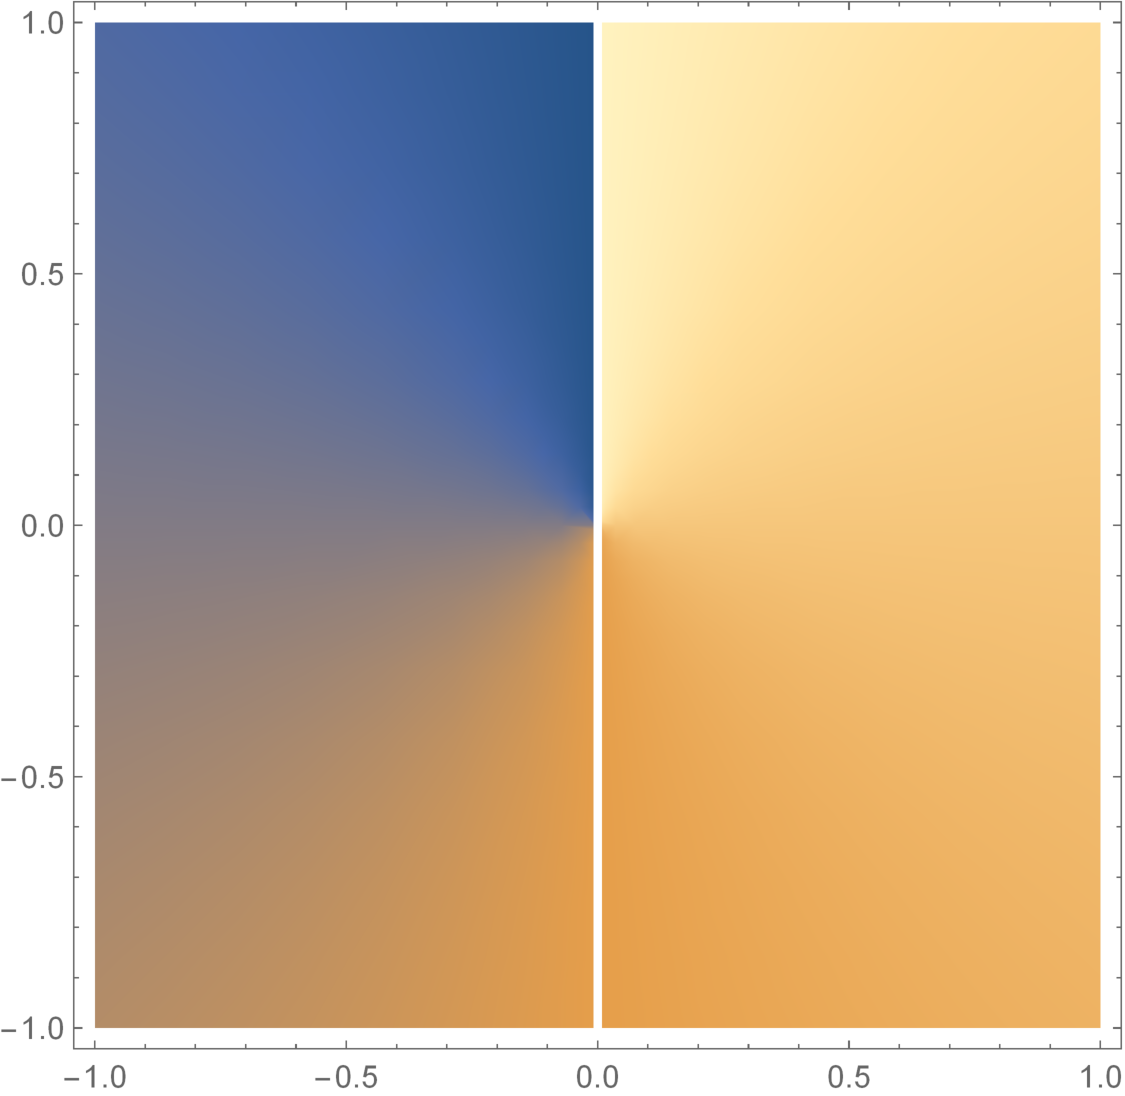
\includegraphics[width=0.5\textwidth]{chern-simons-single-flux-potential.pdf}
    \caption{Density plot of $\chi$ on the $x$-$y$ plane. Obtained by \href{chern-simons-single-flux.nb}{this Mathematica notebook}.}
    \label{fig:single-flux-potential}
\end{figure}

One more thing we need to do is to find the EFT for the $1 / \nu$ FQHE driven by the external electromagnetic field.
The EOM of such a theory must result in something like \eqref{eq:iqhe-eom}, 

\section{Chern-Simons description of the $\mathbb{Z}_2$ topological order}

% TODO: K matrix is 2 sigma^x

We can say that we are in a ``good'' representation of the $\mathbb{Z}_2$ topological order, since there is no 
quantum fluctuation here. The microscopic model of a topological order, if in the language of the ``real'' 
degrees of freedom (i.e. degrees of freedom like spins or electrons that are ``understandable''), often involves strong quantum fluctuation to generate an emergent gauge theory.
A string-net model describes the same universality class yet can be solved exactly, and therefore has 
strong quantum fluctuation in the representation of ``real'' degrees of freedom but no strong quantum 
fluctuation in the representation of operators like $A_i$ or $B_p$. The nonlocality and long-range entanglement 
is hidden in the definition of these seemingly simple operators. A TQFT description further hides the 
quantum fluctuation in the microscopic details.

\bibliographystyle{plain}
\bibliography{../topological-seminar-fd/field-theory,topological-order} 

\end{document}